\chapter{The Bayesian GLLAMM for binary outcomes} \label{chap:framework}

The Generalized Linear Latent and Mixed Model (GLLAMM) is a framework that unifies a wide range of latent variable models. Developed by Rabe-Hesketh, Skrondal and partners \cite{Rabe_et_al_2004a, Rabe_et_al_2004b, Rabe_et_al_2004c, Skrondal_et_al_2004a, Rabe_et_al_2012}, the method was motivated by the need of a Multilevel Structural Equation Model (MSEM, SEM) that accommodates for unbalanced data, noncontinuous responses and the use of cross-level effects among latent variables. The authors focused its development mainly from the frequentist perspective, however, they offered a general guidance on implementing the models under the bayesian framework (see \citet{Skrondal_et_al_2004a}).

In this section we are going to motivate the model from an example. We will start describing the model from the IRT perspective, to later move into the unifying and easily extendable GLLAMM framework.


\section{Model motivation} \label{sect:motivation}

Consider a large standardized assessment composed of three sub-test designed to evaluate the reading comprehension, mathematical reasoning, and pedagogical knowledge of individuals; where each sub-test is composed of several dichotomously scored items. 

Focusing now on the first sub-test, the items were designed to measure three hierarchically nested sub-dimensions of reading comprehension: literal, inferential, and reflective abilities. Therefore, the items ``point-out" only to one of the aforementioned scales. Furthermore, its is assumed that the three sub-dimensions are all that is needed to measure the reading comprehension ability, effectively making this scale the highest level latent variable in the model, similar to a hierarchical Confirmatory Factor Analysis (CFA). Finally, the items are bundled in groups of five to a common text or passage, i.e. testlets, that provides the stimulus over which the individual will be assessed. Figure \ref{fig:design} shows the path diagram of the hypothesized dimensional structure, for a hierarchical cross-classified IRT model corresponding with the aforementioned instrument design.

\begin{figure}[h] \label{fig:design}
	\centering
	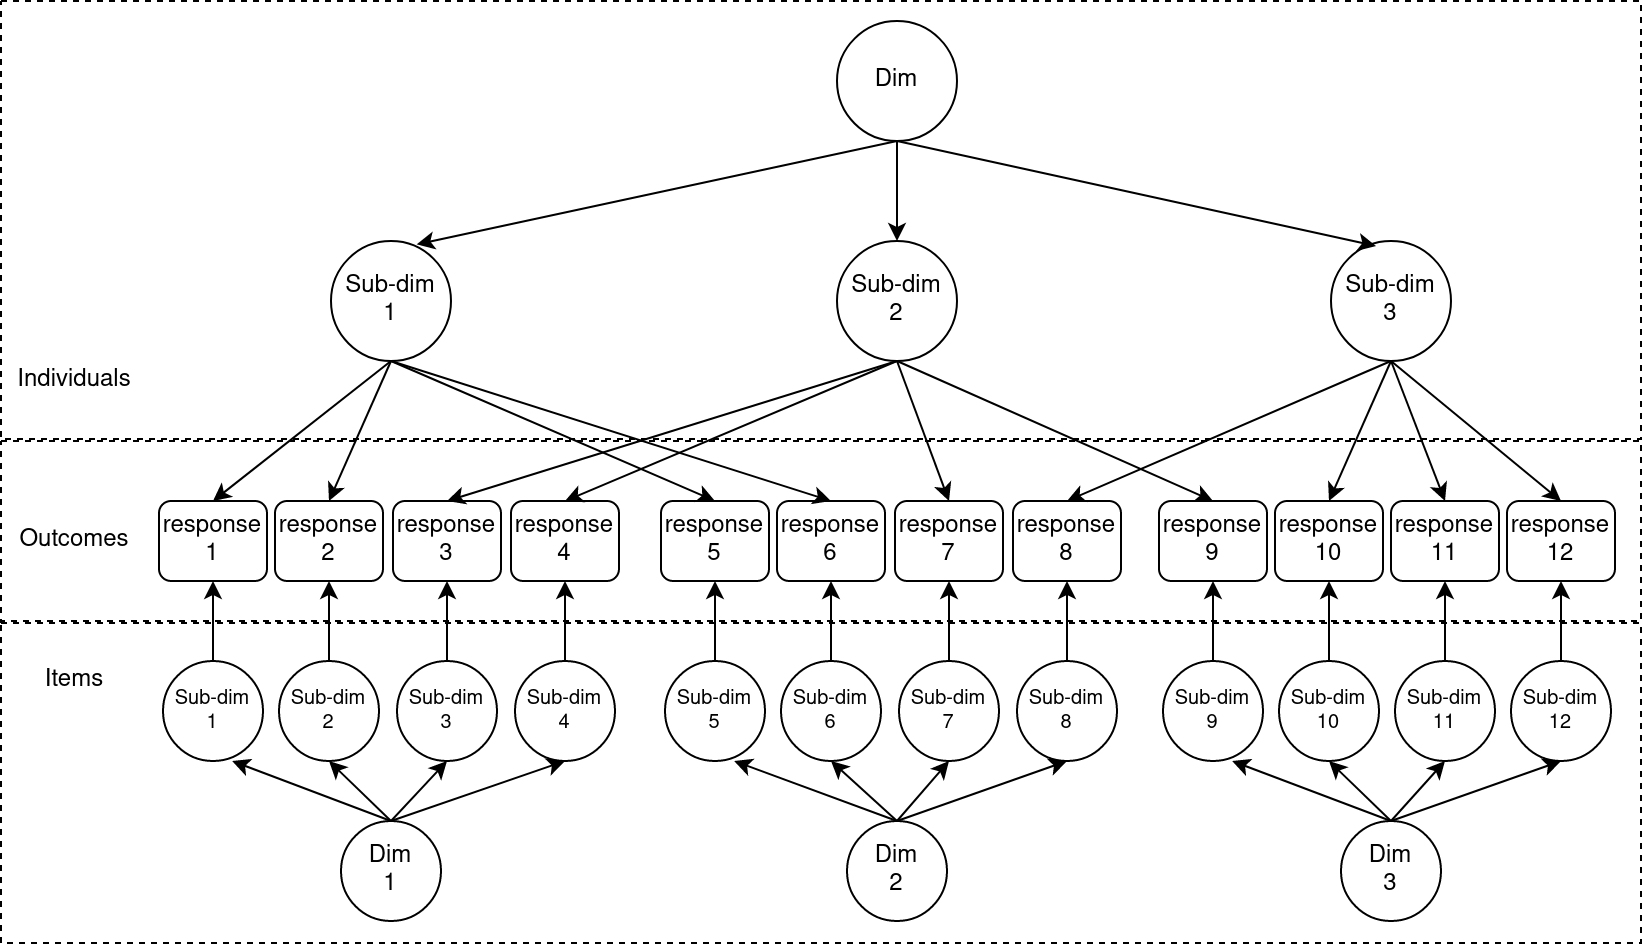
\includegraphics[width=0.85\textwidth]{instrument_design.png}
	\caption{Path diagram of the dimensional structure for a hierarchical cross-classified IRT model, corresponding to the aforementioned instrument design. Squares represent dichotomous manifest variables, and circles represent latent variables. The figure is based on reduced set of items, while errors and scales of the latent variables are not represented. Different sub-dimensions in the individuals block represent the literal, inferential and reflective abilities, while in the items blocks represent the items' difficulties. The dimensions in the individuals block represent the reading comprehension ability, while in the items block represent the multiple testlets.}
\end{figure}

With the purpose of providing an easier motivation of the model, we will not consider yet the clustering effects; however, later in the presentation we will show how easy is to introduce them in the model. Just for future reference, under this example, one expects to observe clustering effects either due to the fact that the evaluation is not mandatory, or because is hypothesized that individuals from different regions did not have the same educational opportunities, effectively causing a regional clustering.

The model departs from the traditional multivariate framework for formulating factor and structural models, i.e. a wide data format\footnote{ The subject’s repeated outcomes are stored in a single row, with multiple response vectors. Moreover, different variables are appended column-wise to the outcome data. }, and adopts a univariate approach, i.e. a long data format\footnote{ The subject’s repeated outcomes are stored in a single ``stacked" response vector with as many rows as there are repeated measurements. Moreover, different variables are appended column-wise to the outcome data, distinguished from each other, by a design matrix. }. 

Under this setting, the outcomes are modeled at the first level. Additionally, the model consider that each individual is indexed with $j = 1, \dots, J$, where $J$ represents the total number of individuals in the sample, while each item is indexed with $k= 1, \dots, K$, where $K$ defines the total number of items. On the other hand, $I$ will represent the number of levels in the individuals block, and $M_{i}$ will represent the number of latent variables within the same block. From figure \ref{fig:design} we notice that $I=2$ levels, while $M_{2}=3$ and $M_{2}=1$, corresponding to the $3$ dimensions in the first level

Each testlet is identified with $m=1, \dots, M$, where $M$ is the total number of common stimulus (texts or passages). Finally, each sub-dimensions of interest is be indexed by $d=1, \dots, D$ where $D$ is the total number of sub-dimensions of interest. 

Following \citet{Rabe_et_al_2004a, Rabe_et_al_2004b}, the dichotomous items ($y_{jkmd}$) are modeled by a Bernoulli probability mass function $f(\cdot)$, in the following form:
\begin{equation} \label{eq:outcome}
	\begin{split}
		f \left( y_{jkmd}=1 | \pmb{\beta}, \pmb{\lambda}, \pmb{\eta}, \mathbf{X}, \mathbf{Z} \right) &= \pi_{jkmd}^{n} (1-\pi_{jkmd})^{1-n}
	\end{split}
\end{equation}

\noindent where $n$ denotes the number of successes in $n$ independent Bernoulli trials.

\section{Model definition} \label{sect:definition}

defined the model as comprised of two parts: (i) the response, and (ii) the latent structure. The response part of is set to directly model the outcome, whereas, the latent structure is responsible of modeling the latent variables.




\subsection{Response model} \label{s_sect:response}

Conditional on the latent variables, the response model is a Generalized Linear Model (GLM) \cite{Nelder_et_al_1989} defined by: (i) a systematic part, composed of a linear predictor and a link function, and (ii) a distributional part. 

\subsubsection{Linear predictor} \label{ss_sect:linear_predictor}
For a model with $L$ levels and $M_{l}$ latent variables at $l>1$ levels, the linear predictor takes the following form:
\begin{equation} \label{eq:linear_predictor}
	v = \mathbf{X} \pmb{\beta} + \sum_{l=2}^{L} \sum_{m=1}^{M_{(l)}} \eta_{m}^{(l)} \mathbf{Z}_{m}^{(l)} \pmb{\lambda}_{m}^{(l)}
\end{equation}

\noindent where $\mathbf{X}$ is a design matrix that maps the parameter vector $\pmb{\beta}$ to the linear predictor, $\eta_{m}^{(l)}$ the $m$th latent variable at level $l$ ($m=1, \dots, M_{(l)}$ and $l=1, \dots, L$), and $\mathbf{Z}_{m}^{(l)}$ a design matrix that maps the vector of loadings $\pmb{\lambda}_{m}^{(l)}$ to the $m$th latent variable at level $l$.

Note that wo do not use subscripts for the units of observation at different levels. This decision was made with the purpose of avoiding the use of mathematical definitions with large number of subscripts. However, a careful reader should consider that equation (\ref{eq:linear_predictor}) rest on the assumption that each unit is identified at their appropriate level. For special cases of multilevel SEM, and their use of subscripts, refer to Appendix \ref{appA:additional}.

\subsubsection{Links and Distributions} \label{ss_sect:link_dist}
As in the GLM framework, the model "links" the expectation of the conditional response, to the linear predictor, through a inverse-link function $h(\cdot)$, in the following form: 
\begin{equation} \label{eq:response_function}
	\mu = E[y | \mathbf{X}, \mathbf{Z}, \pmb{\eta}] = h(v)
\end{equation}

\noindent where equation (\ref{eq:response_function}) can be re-written in terms of the link function $g(\cdot) = h^{-1}(\cdot)$:
\begin{equation} \label{eq:link_function}
	g(\mu) = g(E[y | \mathbf{X}, \mathbf{Z}, \pmb{\eta}]) = v
\end{equation}

\noindent with $\pmb{\eta}=\left[\eta^{(2)T}, \dots, \eta^{(L)T}\right]^{T}$ and $\mathbf{Z}=\left[\mathbf{Z}^{(2)T}, \dots, \mathbf{Z}^{(L)T}\right]^{T}$, as the "stacked" vector of latent variables, and the "stacked" design matrices of explanatory variables, for all $L$ levels, respectively. Additionally, $\pmb{\eta}^{(l)}=\left[\eta_{1}^{(l)}, \dots, \eta_{M_{(l)}}^{(l)}\right]^{T}$ and $\mathbf{Z}^{(l)}=\left[\mathbf{Z}_{1}^{(l)T}, \dots, \mathbf{Z}_{M_{(l)}}^{(l)T}\right]^{T}$, denotes the vector of latent variables, and the "stacked" design matrix of explanatory variables, at level $l$, respectively.

Finally, the response model specification is complete when we select an appropriate distribution from the family of exponential distributions. The types of responses that can be accommodated by the framework are the following:

\textbf{Dichotomous:} \\
	It results from selecting an appropriate inverse-link function for the expected value of the manifest variable, which describe the probability of endorsing one of the two available categories,
	\begin{equation} \label{eq:link_dich}
		\begin{split}
		\mu &= E[y=1 | \mathbf{X}, \mathbf{Z}, \pmb{\eta}] \\ 
		&= P[y=1 | \mathbf{X}, \mathbf{Z}, \pmb{\eta}] \\
		&= \pi \\
		&= h(\kappa - v)
		\end{split}	
	\end{equation}
	where $\kappa$ is the decision threshold, and $h(\cdot)$ can be defined in three ways:	
	\begin{equation} \label{eq:response_dich1}
		h(x) = 
		\begin{cases}
			exp(x)[1 + exp(x)]^{-1} \\
			\Phi(x) \quad \text{No closed form.} \\
			exp(-exp(x))
		\end{cases}
	\end{equation}
	which corresponds to the logistic, standard normal $\Phi(x)$, and Gumbel (extreme value type I) \textit{cumulative distributions}, respectively. In terms of link functions, the distributions corresponds to the well known logit, probit and complementary log-log link functions, respectively. 
	
	Alternatively, the same parametrization can be achieved using the concept of an underlying latent variable in the form $y^{*} = v + \epsilon^{*}$, where $y = 1$ if $y^{*} \ge \kappa$, and $\epsilon^{*}$ can have a distribution as the ones defined in equation (\ref{eq:response_dich1}). It is important to mention that under this parametrization, the threshold parameters $\kappa$ and the $\pmb{\beta}$ {\color{red} are confounded as they serve similar purposes, so only one would be estimated}.
	
	Finally, the distributional part is defined by a Binomial distribution,
	\begin{equation} \label{eq:dist_dich}
		\begin{split}
		f[y=1 | \mathbf{X}, \mathbf{Z}, \pmb{\eta}] &= \binom{n}{k} \mu^{k} (1-\mu)^{n-k} \\
		&= \binom{n}{k} \pi^{k} (1-\pi)^{n-k}
		\end{split}
	\end{equation}

	where $k$ denotes the number of successes in $n$ independent Bernoulli trials.
	



\subsubsection{Heteroscedasticity and over-dispersion in the response} \label{ss_sect:het}

Much like the Generalized Linear Mixed Model framework (GLMM), the GLLAMM allows to model heteroscedasticity, and over- or under-dispersion by adding random effects to the linear predictor, at level $1$. The types of responses, in which such characteristics can be modeled, are the following:
	
\textbf{Dichotomous:} \\
	In a more straightforward way, we model over- or under-dispersion by modifying equation (\ref{eq:link_dich}), to include random intercepts at level $1$, in the following form:
	\begin{equation} \label{eq:link_dich1}
		\begin{split}
			\mu &= P[y=1 | \mathbf{X}, \mathbf{Z}, \pmb{\eta}] \\
			&= \pi \\
			&= h(\kappa - v + \pmb{\alpha}^{T}\mathbf{Z^{(1)}})
		\end{split}	
	\end{equation}
	
	


\subsection{Structural model for the latent variables} \label{s_sect:struct}
The structural model for the latent variables has the form:
\begin{equation} \label{eq:structural_model}
	\def\sss{\scriptstyle}
	\setstackgap{L}{12pt}
	\def\stacktype{L}
	\pmb{\eta} = \stackunder{\mathbf{B}}{\sss (M \times M)} \stackunder{\pmb{\eta}}{\sss (M \times 1)} + \stackunder{\pmb{\Gamma}}{\sss (M \times Q)} \stackunder{\mathbf{W}}{\sss (Q \times 1)} + \stackunder{\pmb{\zeta}}{\sss (M \times 1)}
\end{equation}
where $\mathbf{B}$ and $\pmb{\Gamma}$ are parameter matrices that maps the relationship between the latent variables $\pmb{\eta}$, and the vector of "stacked" covariates $\mathbf{W}$, respectively; $\pmb{\zeta}$ is a vector of errors or disturbances, and $M = \sum_{l} M_{l}$. Notice that while equation (\ref{eq:structural_model}) resembles to single-level structural equation models, the main difference lies in the fact that the latent variables may vary at different levels. Additionally, considering that $\pmb{\eta}$ has no feedback effects, and it is permuted and sorted according to the levels, $\mathbf{B}$ is defined as a strictly upper triangular matrix. In this regard, it is important to mention that,
\begin{enumerate}
	\item The absence of feedback loops implies that the method deals with non-recursive models, i.e. none of the latent variables are specified as both causes and effects of each other \cite{Kline_2012}; {\color{red} this in turn allows the easy estimation of the model parameters}.
	
	\item The strictly upper triangular structure reveals that the framework does not allow latent variables to be regressed on lower level latent or observed variables, as such specification is more related to the use of formative, rather than reflective, latent variables. For a detail explanation on the topic refer to \citet{Edwards_et_al_2000}.
\end{enumerate}
Notice, however, the previous restrictions does not hinder the ability of the method to model contextual effects, after controlling the lower level compositional effects. For examples of such refer to Appendix \ref{appA:additional}.



\subsection{Distribution of the latent variables} \label{s_sect:dist_lv}
Finally, to fully specify the framework, and provide a scale for the latent variables, we have to make assumptions for either the distribution of the disturbances $\pmb{\zeta}$ or the latent variables $\pmb{\eta}$. If our research interest lies in the structural equation model, it is more convenient to make assumptions for the distribution of the disturbances; otherwise, we make assumptions for the distributions for the latent variables. 

Furthermore, as in the hierarchical framework, it is assumed the latent variables at different levels are independent, whereas latent variables at the same level may present dependency. In that sense, we presume all latent variables at level $l$ to have a multivariate normal distribution with zero mean and covariance matrix $\Sigma_{l}$, i.e. $\pmb{\eta}^{(l)} \sim MVN(\mathbf{0}, \pmb{\Sigma}_{l})$. It is important to emphasize that, while the multivariate normal distribution is widely used in these settings, it is not the only distribution that can be assumed. \citet{Rabe_et_al_2003a} have provided evidence that it can be even left unspecified, by using non-parametric maximum likelihood estimation.



\subsection{Model identification} \label{sect:identification}
{\color{red}(work in progress) \\
	
The structure of the latent variables is specified by the number of levels L and the number of latent variables Ml at each level. A particular level may coincide with a level of clustering in the hierarchical dataset. However, there will often not be a direct correspondence between the levels of the model and the levels of the data hierarchy.

}




\section{The bayesian estimation}


The practical use of GLLAMM requires the estimation of the parameters associated with the items and the individuals' latent abilities. These can be obtained within two frameworks: the classical (frequentist), and the bayesian. The current chapter center its attention on describing the bayesian framework using the Markov Chain Monte Carlo method (MCMC). For a full development of GLLAMM under the frequentist estimation framework refer to \citet{Rabe_et_al_2004a, Rabe_et_al_2004b, Skrondal_et_al_2004a, Rabe_et_al_2012}.


\subsection{Benefits and shortcomings}

The reasons on why bayesian statistics is attractive to perform the estimation of the parameters of any model, and especially under the GLLAMM framework, are:

\begin{enumerate}
	\item The bayesian estimates are at least as good as the frequentist estimates \cite{Baker_1998, Wollack_2002, Hsieh_2010}. 
	
	\item It is built on a simulation-based estimation method, therefore, it can handle all kinds of priors and data-generating processes \cite{Fox_2010}. This is especially useful with highly complex and over-parameterized models, where other methods are unfeasible or work poorly \cite{Baker_1998, Kim_1999}. 
	
	\item The model definitions, i.e. the likelihood for the data and priors for the parameters, are used to estimate the corresponding posterior distributions. However, the definitions can also be used in a generative way, i.e. simulate observations, allowing us to test the ability of the method/data to recover the parameters of interest \cite{McElreath_2020}.
	
	\item It allow us to integrate prior beliefs or knowledge about the parameters beyond the observed responses \cite{Fox_2010, Skrondal_et_al_2004a}. This is especially useful when we have issues of non-convergence or improper estimation of the parameters under the Maximum Likelihood methods (ML). Examples of these cases are:
	
	\begin{enumerate}
		\item Estimating abilities when individuals have null scores or aberrant response patterns, i.e. examinees that answered some relatively difficult and discriminating items correctly, while answering some of the easiest incorrectly. \cite{Hambleton_et_al_1991a, Azevedo_2003}.
		
		\item Estimating parameters that need to be confined to a permitted parameter space, e.g. the estimation of positive unique factors variances, where the opposite is known as ‘Heywood cases’ \cite{Martin_et_al_1975}
		
		\item Estimating parameters under a sparse data structure, where the asymptotic theory is unlikely to hold \cite{Fox_2010};
		
	\end{enumerate}
	
\end{enumerate}

\noindent Finally, in terms of shortcomings, the bayesian framework has the following inconveniences:

\begin{enumerate}	
	\item It exposes the user to arbitrary" decisions about the running of the chains, e.g. how many iterates does the chain need to achieve precise estimates?, what is the right size for the burn-in and warm-up phases?, how should the thining procedure be performed? \cite{Skrondal_et_al_2004a}. 
	
	\item The user has many options to assess if the chain achieves stationarity, convergence or good mixing, and most of them are visual. This makes it hard to assess if the chain converges to a proper distribution \cite{Gelman_et_al_1996}.
	
	\item The procedure makes it hard to discover parameters' lack of identification \cite{Skrondal_et_al_2004a}. Inadequate mixing of the chain could lead us to think unidentified parameters have been estimated with precision, when in fact they have a `flat' posterior \cite{Keane_1992}.
	
	\item Sometimes the geometry of the model makes it hard to find proper solutions for the parameter space. This is especially true in hierarchical models. Under this circumstances, the scientist needs to re-parameterize the model to a non-centered form, i.e. remove the dependence of the parameters on other sampled parameters \cite{Gorinova_et_al_2019}. In those cases, the complexity of the transformation limit the ability of the scientist to communicate/share the implementation \cite{McElreath_2020}.
	
	\item The procedure requires more time to achieve a proper solution, compared to the classical methods. This is especially true in models with high complexity \cite{Tarazona_2013, Rivera_2019}.
	
\end{enumerate}

\noindent Although some of the shortcomings has made the use of bayesian methods a "controversial" issue, most of these already have an acceptable solution. 

For the first point, a popular approach to solve the issues is to use a large number of iterates, or multiple chains with different initial states. This is mostly applicable under the Metropolis-Hastings and Gibbs sampling methods. However, as we will see in section \ref{sect:comp_imp}, the Hamiltonian Monte Carlo method (HMC) \cite{Betancourt_et_al_2013} implements a different sampling mechanism that is less reliant on these decisions. 

About the second shortcoming, it is well accepted that the visual assessment of stationarity and convergence is easier, and this procedure usually has additional support from statistics like \texttt{Rhat} \cite{Gelman_et_al_2014}. On the contrary, a visual evaluation of `good' mixing remains as a hard task. A popular approach to increase the possibility of a well mixed chain is to change the geometry of the model \cite{McElreath_2020}. However, the implementation of the approach does not necessarily ensure the required property.

On the third point, the most common solution is to use regularizing priors, i.e. priors that are more `skeptical' of wider parameter spaces \cite{McElreath_2020}. However, it is important to mention, there are scenarios where one can achieve poor parameter estimates, even in the presence of `enough' data and regularizing priors, e.g. the estimation of the variance parameters in random effects models \cite{Skrondal_et_al_2004a}, but this is also applicable to the classical estimation procedures.

Finally, the fourth and fifth points can be considered as the `price' a scientist has to pay to be able to fit complex models, that are in more accordance with the observed data generating processes.


\subsection{Bayesian framework}

\subsubsection{Prior distribution}

\subsubsection{Initial start}

\subsubsection{Likelihood}

\subsubsection{Posterior distribution}


\section{Computational implementation} \label{sect:comp_imp}

{\color{red} (work in progress) \\
	see \\
	- Gelman et al (2011) - Handbook of Markov Chain Monte Carlo\\
	- McElreath (2020) - Statistical Rethinking
	
	Rethinking: Warmup is not burn-in. Other MCMC algorithms and software often discuss burn-
	in. With a sampling strategy like ordinary Metropolis, it is conventional and useful to trim off the
	front of the chain, the “burn-in” phase. This is done because it is unlikely that the chain has reached
	stationarity within the first few samples. Trimming off the front of the chain hopefully removes any
	influence of which starting value you chose for a parameter. 156
	But Stan’s sampling algorithms use a different approach. What Stan does during warmup is quite
	different from what it does after warmup. The warmup samples are used to adapt sampling, to find
	good values for the step size and the number of steps. Warmup samples are not representative of
	the target posterior distribution, no matter how long warmup continues. They are not burning in,
	but rather more like cycling the motor to heat things up and get ready for sampling. When real
	sampling begins, the samples will be immediately from the target distribution, assuming adaptation
	was successful.
	
}


The procedure will be with the aid of \texttt{Stan} \cite{Stan2020} and \texttt{R} \cite{R2015, RStan2020} to retrieve . \\


\newpage
{\color{red}(to be erased) \\


\section{Relationship with other modeling schemes}

From section \ref{sect:definition}, it is evident that the GLLAMM framework shares some common ground, and even extends, some of the most important modeling schemes, such as the GLM, GLMM, SEM, and the Generalized Latent Model framework, from which the Item Response Theory Model (IRT) stand out.

\subsection{Generalized Linear and Mixed Models}

The Generalized Linear Model (GLM) framework, presented by \citet{Nelder_et_al_1972}, and further developed by \citet{Nelder_et_al_1989}, was formulated with the purpose of expanding the linear regression model to other types of responses, like dichotomous, and counts. The scheme generalizes the linear model by "linking" the mean response variable to a linear predictor, and further allowing the magnitude of the variance, of each measurement, to be a function of its predicted value. Finally, the scheme is fully defined after selecting a distribution, from the exponential family, to model the distribution of the response variable.

As expressed in the previous paragraph, the GLM framework fixes the relationship of the modeled dispersion to the mean value, e.g. in the counts case $\mu = \lambda$, and $v(\mu) = \lambda$. However, in practice, this assumption is often violated as the data can present over- or under-dispersion. Even in the continuous response case, where the mean and variance function are not related, the model assumes that the errors are homoscedastic, identical and independently distributed. However, this assumption is often violated when the units of analysis are correlated or belong to a cluster, e.g. when students are nested in schools, and these are further nested in districts or states.

It is important to mention that, while the GLM framework can model heteroscedasticity, over- or under-dispersion, it does it in a way that does not allow them to be dependent on covariates, something that might be of interest for a researcher.

Given the restrictions of GLM, the Generalized Linear Mixed Model (GLMM) framework was developed. The method handled the hierarchical or clustered structure in the data, and in doing so, indirectly modeled the heteroscedasticity, over- or under-dispersion by adding latent variables, called "random effects”, to the linear predictor. Under the framework, the random variables are often interpreted as the effects of unobserved covariates, at different levels, that induce dependence among lower-level units \cite{Rabe_et_al_2012}, and can be further explained by additional observed covariates. 

From the previous description, it is easy to notice that the GLLAMM framework uses the same generalization and distributional assumptions, for the response variables, as the GLM; while it borrows the idea of modeling the hierarchical or clustered structure in the data, by including random effects; from the GLMM. However, it is clear that the GLLAMM further generalize both, by allowing the framework to model measurement error at different levels of the hierarchy in the data.



\subsection{Structural Equation Models}

Considering that, in practice, researchers are often faced with variables that cannot be measured directly or reflect measurement error, e.g. intelligence, depression, student abilities, among other; the statistical literature was instigated to develop methods that can handle such data characteristics. 

{\color{red}(work in progress) \\
The disciplinary seeds of Structural Equation Models (SEM) were set by \cite{Spearman_1904}, with a factor model on intelligence testing, passing through \cite{Wright_1920}, with a path analysis in the context of genetic and biology, to finally land in the sociological field, with the work of \cite{Blalock_1961}.

to include several features of the previous modeling scheme, i.e. generalized linear mixed models, the framework is characterized by the fact that it is a method that can impute relationships between unobserved factors or latent variables, and observable or manifest variables. Under this framework, it is assumed that such "common factors" are responsible for the variation and dependence in the manifest variables.

mention Factor Models, Item Response Theory and Generalized Latent Models, and Multilevel Structural Equation Models
\ref{s_sect:dist_lv}


multilevel structural equation models represent a synthesis between multilevel regression models and structural equation models. Considering that 
}


\section{Advantages and Disadvantages}
}